% labels:
% cap:implementacao
% sec:arq
% sec:exp

\externaldocument{fundamentos}

%% ---------------------------------------------------------------------------- %
\chapter{Implementação}
\label{cap:implementacao}
%% ---------------------------------------------------------------------------- %

\section{Ambientes}
\label{sec:envs}

%[1]https://papers.nips.cc/paper/3964-double-q-learning
%[2]https://arxiv.org/pdf/1511.06581.pdf

Antes de apresentar as arquiteturas das redes utilizadas e como os treinamentos foram feitos, serão formalizados os ambientes e os \hyperref[sec:mdp]{MDPs} que os modelam.

\subsection{\textit{Gridworld}}
\label{sec:env_gw}

Os estados $S$ são o mapa em que o agente está inserido com o agente em uma das posições possíveis.
Portanto, o número de estados existentes é igual ao número de espaços válidos.
As ações possíveis $A$ são mover-se para o espaço acima, abaixo, a direita ou a esquerda contanto que seja válido.
É possível o agente decidir mover-se para um espaço inválido, mas isso faz apenas com que ele não saia do lugar.
Os valores das recompensas $R(S,A)$ são definidas pelo desenvolvedor do ambiente.
O objetivo é um estado terminal de recompensa positiva, a armadilha é um estado terminal de recompensa negativa, e estados não-terminais podem gerar recompensas não-nulas se o desenvolvedor quiser.
As probabilidades de transição $P(S,A,S')$ são as probabilidades de o agente estar em um determinado espaço do mapa (estado $S$) e, a partir do movimento para algum dos espaços adjacentes (ação $A$), chegar a algum outro espaço do mapa (estado futuro $S'$).
Não existe aleatoriedade no movimento do agente, pois ele sempre se desloca para a direção que escolheu, não sendo possível, por exemplo, mover-se para a direita quando a ação de mover-se para cima for escolhida.

Os experimentos foram feitos no \textit{Frozen Lake} do Gym, pois ele funciona da mesma forma que o \textit{Gridworld} conforme descrito acima, com a exceção de os movimentos não serem determinísticos, ou seja, é possível o agente escolher mover-se para um lado mas deslocar-se para outro.
Para que ele funcionasse como o desejado, essa aleatoriedade foi removida.
No caso deste trabalho, o mapa é de tamanho 10x10 com 8 armadilhas, 1 objetivo e nenhum espaço inválido, ou seja, há 100 espaços possíveis.
O objetivo gera recompensa de valor 1000, as armadilhas de valor -200, e estados não terminais de -1.
O mapa em que os experimentos foram feitos está representado pela imagem \ref{fig:env_grid}.

\begin{figure}[h!]
  \centering
  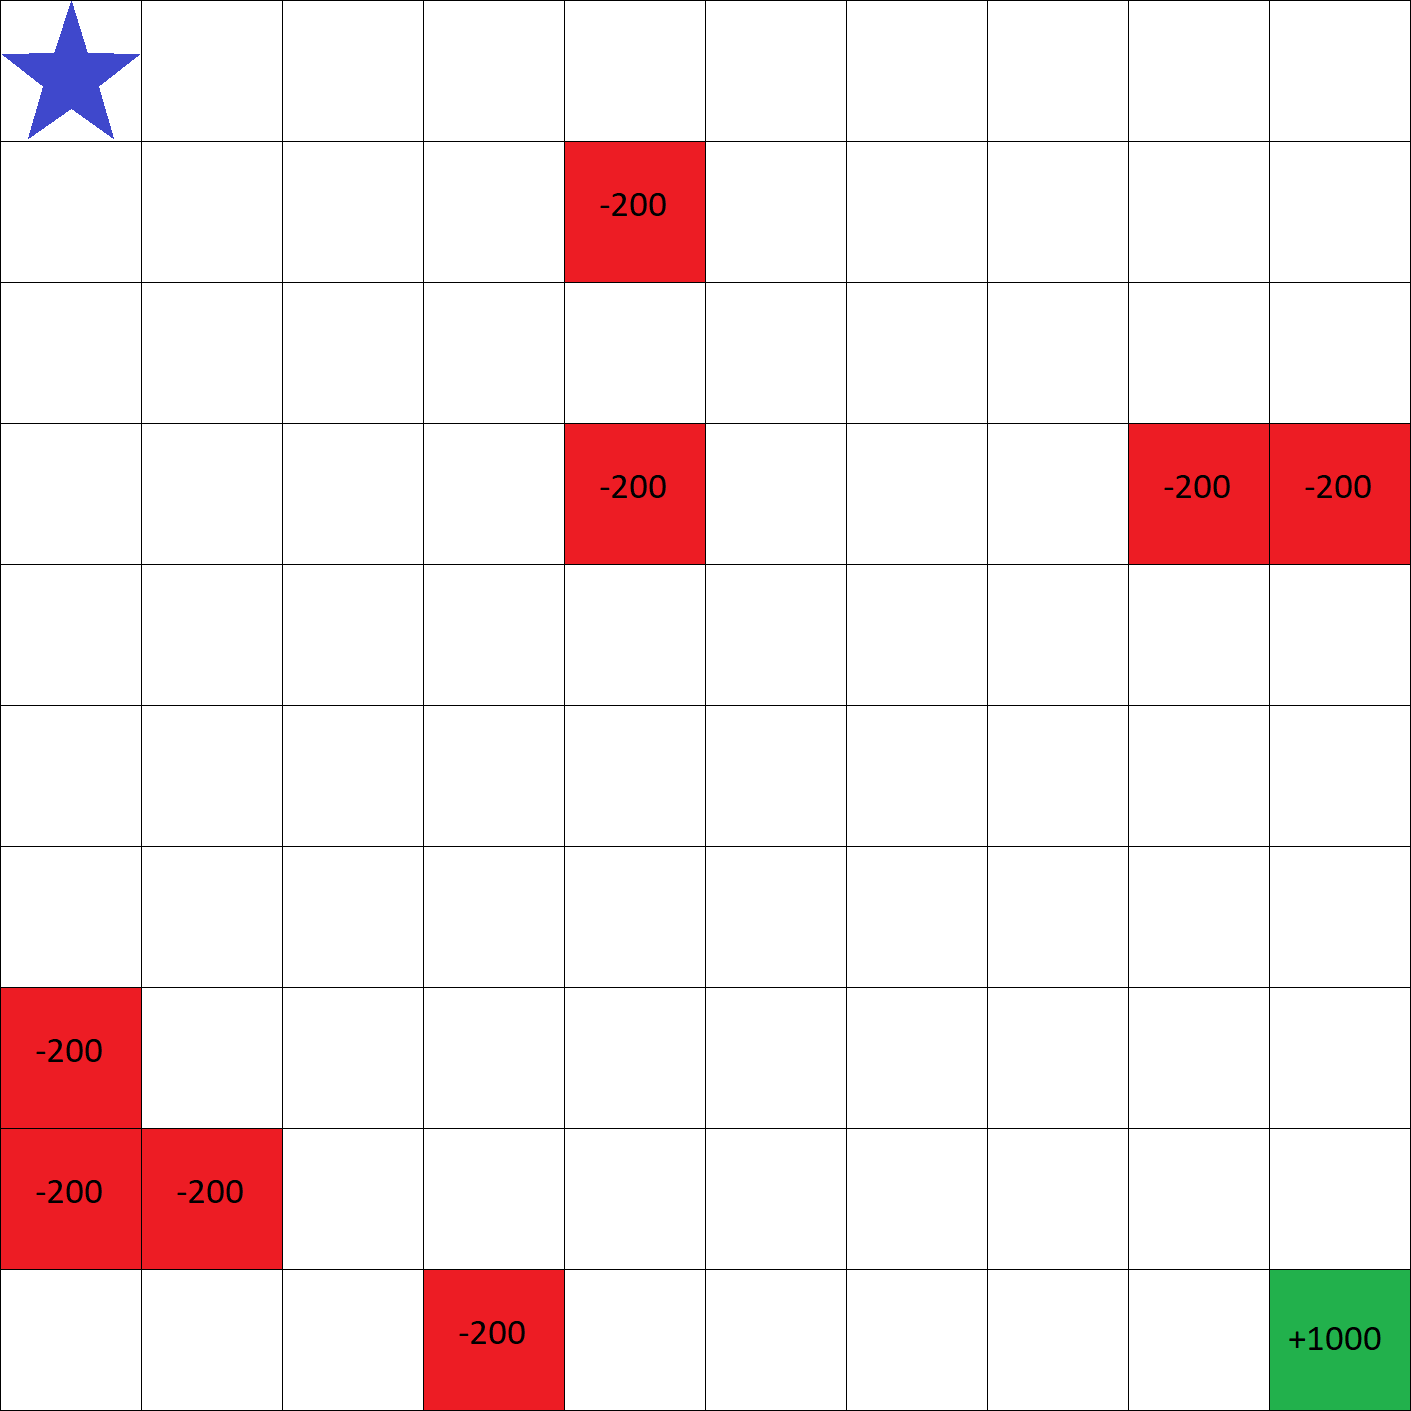
\includegraphics[scale=.2]{env_gridworld}
  \caption{Mapa utilizado para os experimentos. A estrela azul indica a posição inicial do agente, o verde com +1000 representa o objetivo, e os vermelhos com -200 as armadilhas. Não há espaços inválidos.}
  \label{fig:env_grid}
\end{figure}

\textit{Gridworld} é o ambiente mais simples estudado neste trabalho, pois possui poucas regras, estados possíveis, e ações válidas em cada um deles.

\subsection{\textit{Pong}}
\label{sec:env_pong}

Os estados $S$ são a tela do jogo, representada por matrizes de pixels de três dimensões: altura, largura, e canais de cor.
As ações possíveis $A$ são mover a barra que o jogador controla para cima ou para baixo.
As recompensas $R(S,A)$ são recebidas quando a bola chega ao fim da tela do lado esquerdo ou direito, gerando uma positiva se chegar do lado do adversário, e negativa se chegar do lado do jogador.
%As recompensas $R(S,A)$ são de +1 ponto se fizer a bola chegar ao fim da tela do lado do oponente e de -1 ponto se a bola chegar ao fim da tela do lado do jogador.
As probabilidades de transição $P(S,A,S')$ são as probabilidades de o jogo estar em um estado $S$, por exemplo com a bola sendo rebatida pelo jogador, e transitar para algum outro estado futuro $S'$, como marcar um ponto, após tomar uma ação $A$, como mover a barra para cima.
\textit{Pong} é um jogo determinístico no sentido que não existe aleatoriedade na consequência das ações do jogador: se a bola colidir com a barra sempre no mesmo lugar, ela sempre será retornada na mesma direção com a mesma velocidade; marcar ponto sempre aumenta a pontuação do jogador em um.
Por outro lado, existe um oponente contra o qual se está jogando e cujo comportamento configura um elemento de aleatoriedade no ambiente.
Além disso, o jogador não conseguir rebater a bola como gostaria por falta de precisão também se aproxima de um elemento desse tipo.

Neste trabalho, o \textit{Pong} foi emulado pelo Gym, que utiliza o emulador de Atari 2600, Stella \footnote{\url{https://stella-emu.github.io/}}.
Nessa versão, os estados são compostos por 210x160 pixels, com cada um podendo assumir 128 cores diferentes por combinações dos valores dos 3 canais de cor.
Isso equivale a 33600 pixels e, portanto, $128^{33600}$ estados, com apenas uma parcela sendo realmente possível.
A recompensa por marcar ponto é de +1 e a de o oponente marcar ponto é de -1.
Como o jogo termina quando um dos lados alcança 21 pontos, a pontuação final varia de -21 até +21 inclusos.

\begin{figure}[h!]
  \begin{minipage}[b]{.5\textwidth}
  \centering
  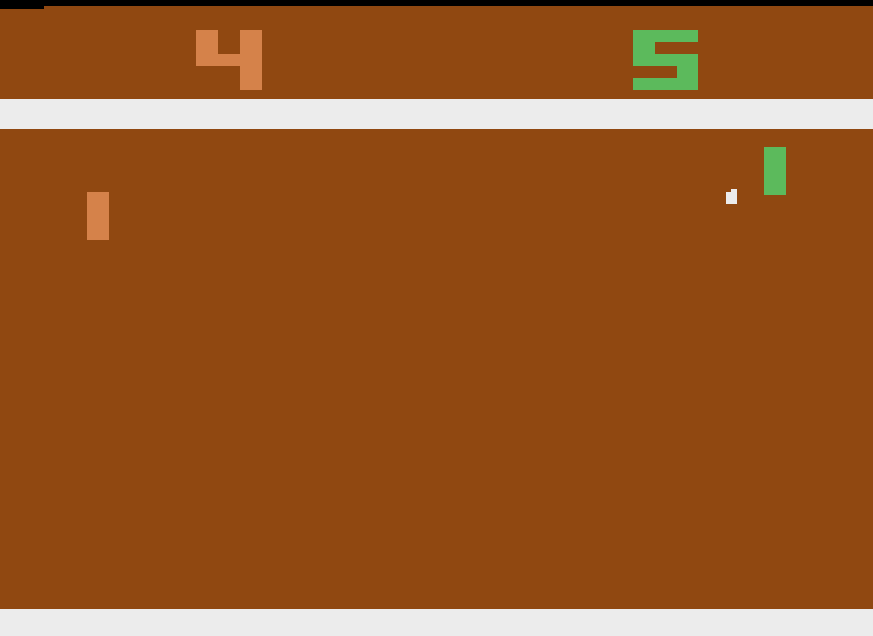
\includegraphics[scale=.25]{pong_example01}
  %\caption{Exemplo de tela do jogo. O números no topo da tela são pontuação e quantidade de vidas respectivamente. A nave, no centro, está atirando. Asteroides espalhados pela tela.}
  \end{minipage}
  \hfill
  \begin{minipage}[b]{.5\textwidth}
  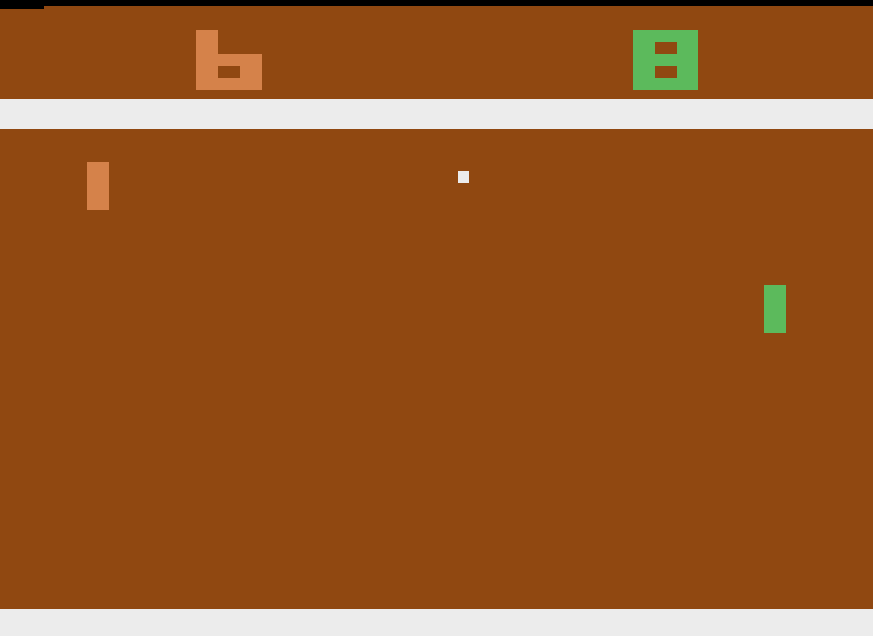
\includegraphics[scale=.25]{pong_example02}
  %\caption{Exemplo de tela do jogo. A nave acaba de destruir um asteroide de menor tamanho e está recebendo uma recompensa de 100 pontos por isso. Asteroides podem ter diversas cores.}
  \end{minipage}
  \caption{Exemplos de tela do jogo no emulador de Atari 2600, Stella. Nestas imagens, o jogador controla a barra verde, do lado direito da tela, enquanto a IA criada pelos desenvolvedores do jogo controla a barra laranja, do lado esquerdo da tela. O ponto branco entre elas é a bola, as barras brancas horizontais que estendem desde o lado equerdo até o lado direito da tela representam os limites superior e inferior do campo, e os números no topo indicam a pontuação de cada jogador.}
\end{figure}

\textit{Pong} é o ambiente de complexidade intermediária estudada neste trabalho, pois possui poucas regras, grande espaço de estados, e poucas ações possíveis em cada um deles.

\subsection{\textit{Asteroids}}
\label{sec:env_asteroids}

Os estados $S$ são a tela do jogo, representada por matrizes de pixels de três dimensões: altura, largura, e canais de cor.
As ações possíveis $A$ são mover-se para frente, girar no sentido horário, girar no sentido anti-horário, mover-se no hiper-espaço (se teletransportar para algum lugar aleatório da tela), e atirar para frente.
As recompensas $R(S,A)$ são recebidas por destruir os asteróides, com o maior valendo menos pontos e o menor valendo mais pontos, podendo ser obtidas tanto atirando neles quanto colidindo, não havendo recompensa negativa pela perda de vida.
%As recompensas $R(S,A)$ são de 20 pontos por destruir um asteróide grande, 50 pontos por destruir um médio e 100 pontos por destruir um pequeno, podendo ser obtidas tanto atirando neles quanto colidindo, não havendo recompensa negativa (penalidade) por perda de vidas.
As probabilidades de transição $P(S,A,S')$ são as probabilidades de o jogo estar em um estado $S$, por exemplo o inicial em que o jogador tem zero pontos e todas as vidas, e transitar para algum outro estado futuro $S'$, como destruir algum asteroide e receber pontos por isso, após tomar uma ação $A$, como atirar para frente.
Assim como em \textit{Pong}, \textit{Asteroids} é um jogo determinístico no sentido que não existe aleatoriedade na consequência das ações do jogador: se ele fizer um disparo, o tiro seguirá reto durante um certo tempo até desaparecer ou atingir um asteroide; cada tamanho de asteroide sempre aumenta a pontuação do jogador pela mesma quantidade quando destruído.
Os fatores mais próximos de aleatoriedade existentes no jogo são o jogador ignorar, desconhecer, abstrair e/ou não perceber partes do jogo, como a posição dos asteróides.

Neste trabalho, o \textit{Asteroids} foi emulado pelo Gym-Retro, que utiliza o emulador de Atari 2600, Stella.
Como esta versão também é a do Atari 2600, o número de estados possíveis é uma parcela de $128^{33600}$ assim como no \textit{Pong}.
A recompensa por destruir um asteróide grande é de 20 pontos, de um médio é de 50 pontos, e de um pequeno é de 100 pontos.
O jogador começa com 4 vidas e recebe uma nova a cada 5000 pontos obtidos.
O único estado terminal nativo do jogo ocorre quando todas as vidas são perdidas.

\begin{figure}[h!]
  \begin{minipage}[b]{.5\textwidth}
  \centering
  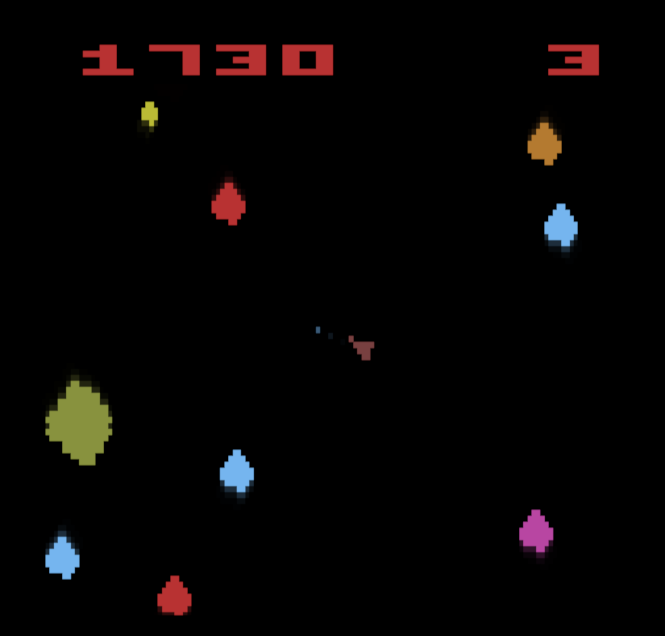
\includegraphics[scale=1.41]{asteroids_example01}
  %\caption{Exemplo de tela do jogo. O números no topo da tela são pontuação e quantidade de vidas respectivamente. A nave, no centro, está atirando. Asteroides espalhados pela tela.}
  \end{minipage}
  \hfill
  \begin{minipage}[b]{.5\textwidth}
  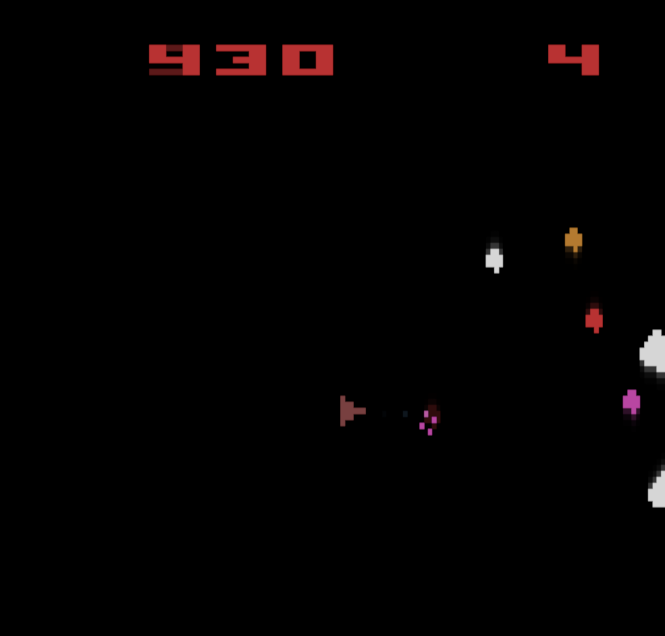
\includegraphics[scale=1.41]{asteroids_example02}
  %\caption{Exemplo de tela do jogo. A nave acaba de destruir um asteroide de menor tamanho e está recebendo uma recompensa de 100 pontos por isso. Asteroides podem ter diversas cores.}
  \end{minipage}
  \caption{Exemplos de tela do jogo no emulador de Atari 2600, Stella. O número no canto superior esquerdo é a pontuação e o no canto superior direito é a quantidade de vidas restante que o jogador tem. A nave é o triângulo no meio da tela, o ponto azul próximo dela na imagem da esquerda é um tiro e o restante é asteroide. Na imagem da direita, os quatro pequenos pontos rosas próximos da nave são um asteroide que acaba de ser destruído.}
\end{figure}

\textit{Asteroids} é o mais complexo dos ambientes estudados neste trabalho, pois possui mais regras que são mais complexas, o maior espaço de estados dentre os três ambientes, e mais ações possíveis. 

%% ---------------------------------------------------------------------------- %

%Agora, será descrito como foi feita a implementação da inteligência artificial.

\section{Arquiteturas das redes}
\label{sec:arq}

Com os ambientes e MDPs formalizado, nesta seção serão descritas as arquiteturas utilizadas nos três ambientes abordados neste trabalho e, em seguida, os respectivos treinamentos feitos.
Todo o código foi escrito em Python3, com as redes neurais sendo construídas utilizando o arcabouço TensorFlow.

\subsection{\textit{Gridworld}}
\label{sec:arq_gw}

%%No caso do \textit{Gridworld}, por ser um ambiente muito diferente do \textit{Pong} e do \textit{Asteroids}, teve uma arquitetura bem mais simples.
Por ter poucos estados e ações possíveis em comparação com o \textit{Pong} e o \textit{Asteroids}, a arquitetura da rede do \textit{Gridworld} foi muito simples.
A rede neural convolucional utilizou uma camada de convolução seguida por uma \textit{fully-connected}, a de saída.
A convolucional tinha 8 filtros de tamanho 2x2, passo 1, função de ativação ReLU e inicializador de Xavier~\cite{pmlr-v9-glorot10a}, enquanto a \textit{fully-connected} tinha um nó de saída para cada ação possível, ou seja, um vetor de tamanho 4, sem função de ativação e inicializada com zeros.
O cálculo de erro foi feito pela função \textit{Huber loss}~\cite{huber_loss} e a otimização pela função \textit{Root Mean Square Propagation}, mais conhecida como RMSProp~\cite{rmsprop}.
A taxa de aprendizado $\alpha$ foi igual a $0.05$;
e o \textit{momentum}, variável que indica o quanto gradientes anteriores devem ser considerados para determinar a direção do movimento, foi igual a $0.1$.
%e probabilidade mínima de se jogar aleatoriamente igual a $0.4$.

\subsection{\textit{Pong}}
\label{sec:arq_pong}

A arquitetura da rede do \textit{Pong} precisou ser mais elaborada para que o agente pudesse obter sucesso.
%%O \textit{Pong}, por ser mais complexo que o \textit{Gridworld}, teve uma arquitetura mais elaborada para se obter sucesso.
%Primeiro, os \textit{frames} são convertidos para escala de cinza.
%Em seguida, partes que não agregam informação para a IA conseguir jogar, como pontuação, foram removidos.
%Depois, o que sobrou da tela é redimensionado para 84x84 pixels.
%Essas etapas servem para reduzir o tempo de processamento ao passar pela rede convolucional e não são feitas no \textit{Gridworld} por não haver necessidade, já que as matrizes de entrada são pequenas.
%Os últimos quatro \textit{frames} vistos são inseridos em uma fila de forma que o agente consiga captar o movimento dos objetos na tela do jogo.
%Esses quatro \textit{frames} enfileirados são enviados juntos para a rede neural, de forma que a entrada tem formato 84x84x4.
Foram utilizadas três camadas de convolução e duas camadas \textit{fully-connected}, sendo a segunda delas a de saída.
A primeira convolucional tinha 32 filtros de tamanho 8x8 e passo 4; a segunda tinha 64 filtros de tamanho 4x4 e passo 2; e a terceira tinha 64 filtros de tamanho 3x3 e passo 1.
A primeira \textit{fully-connected} tinha vetor de saída de tamanho 256; e a segunda tinha um nó de saída para cada ação possível, ou seja, um vetor de tamanho 2.
Todas as camadas utilizaram função de ativação ReLU, com exceção da segunda \textit{fully-connected} que não usou nenhuma, e inicializador de He \footnote{No TensorFlow, esse inicializador é chamado pela função \texttt{variance\_scaling\_initializer()}}~\cite{DBLP:journals/corr/HeZR015} para os pesos.
%A primeira camada de convolução tem 32 filtros de tamanho 8x8 e passo 4, a segunda tem 64 filtros de tamanho 4x4 e passo 2, a terceira tem 64 filtros de tamanho 3x3 e passo 1.
%Todas elas são seguidas da função de ativação ReLU (\textit{Rectified Linear Unit}).
%Depois disso, há uma camada \textit{fully-connected} com 256 unidades e função de ativação ReLU e, por fim, outra camada \textit{fully-connected} com um nó de saída para cada ação possível (dois neste caso), sem função de ativação.
%Todas as camadas utilizam o inicializador de He \footnote{No TensorFlow, esse inicializador é chamado pelo \texttt{variance\_scaling\_initializer()}}~\cite{} para os pesos.
O cálculo de erro foi feito pela função \textit{Huber loss} e a otimização dos pesos pelo RMSProp.
A taxa de aprendizado $\alpha$ foi igual a $0.00025$;
o \textit{momentum} foi igual a $0.1$;
%probabilidade mínima de se jogar aleatoriamente igual a $0.1$;
e $\epsilon$, variável que impede a divisão por zero no cálculo feito pelo RMSProp, igual a $0.1$.
%Após a CNN soltar a ação escolhida, o cálculo de erro é feito pela função \textit{Huber loss} e a otimização dos pesos é feita pelo RMSProp.
%O RMSProp utilizou taxa de aprendizado $\alpha = 0.00025$, momentum = $0.95$ e $\epsilon = 0.01$.
%Foram 298 episódios de treinamento, ou aproximadamente 1 milhão de \textit{frames}, cada um com limite 18000 ações antes de o episódio ser terminado automaticamente, \textit{mini-batches} de tamanho 32, taxa de desconto $\gamma = 0.99$, \textit{buffer} de memória de tamanho 1000000 que foi preenchido com 50000 ações aleatórias antes do treinamento começar.
%O dilema \textit{exploration versus exploitation} utilizou $P_{ini} = 1.0$, $P_{min} = 0.1$ e $decay = 20000$.
%A rede alvo foi atualizada a cada 10000 ações tomadas.

%Além disso, foi utilizada uma técnica simples de pular \textit{frames}~\cite{DBLP:journals/corr/abs-1207-4708} para economizar tempo.
%O agente enxerga a tela e escolhe qual ação tomar a cada 4 \textit{frames} ao invés de em todos os \textit{frames}, repetindo a última ação escolhida nos \textit{frames} pulados.
%Isso acelera o treinamento ao consumir menos tempo por \textit{frame} sem prejudicar muito o aprendizado.
%Esse comportamento é próprio do ambiente\footnote{PongDeterministic-v4 do Gym} utilizado, não havendo partes do código destinadas a isso.

\subsection{\textit{Asteroids}}
\label{sec:arq_asteroids}

O \textit{Asteroids} foi testado com diversas arquiteturas diferentes, mas sem sucessos.
Tentou-se utilizar diferentes números de camadas ocultas, número de filtros, tamanhos e passos, funções inicializadoras e ativadoras, unidades de saída nas camadas \textit{fully-connected}, funções de erro, de otimização e de exploração, taxas de aprendizado, de desconto e de atualização da rede alvo, assim como outras configurações externas à rede neural, como tamanho dos \textit{mini-batches}, do \textit{buffer} de memória e número de episódios de treinamento.
%Tentou-se utilizar diferentes tamanhos de redimensionamento no pré-processamento, números de filtros, tamanhos e passos, funções inicializadoras e ativadoras, unidades de saída nas camadas \textit{fully-connected}, funções de erro, de otimização e de exploração, taxas de aprendizado, de desconto e de atualização da rede alvo, tamanho dos \textit{mini-batches} e do \textit{buffer} de memória.
Por conta da grande gama de hiper-parâmetros a serem ajustados e o tempo consumido para treinar, os testes com este ambiente foram os mais longos.

Para poder demonstrar um exemplo de resultados de treinamento para o capítulo \hyperref[cap:resultados]{Resultados}, foram registrados os resultados de um treinamento cuja rede neural tinha três camadas de convolução e duas \textit{fully-connected}, sendo a segunda delas a de saída.
A primeira convolucional tinha 48 filtros de tamanho 8x8 e passo 4; a segunda tinha 96 filtros de tamanho 4x4 e passo 2; e a terceira tinha 96 filtros de tamanho 3x3 e passo 1.
A primeira \textit{fully-connected} tinha vetor de saída de tamaho 512; e a segunda tinha um nó de saída para cada ação possível, ou seja, um vetor de tamanho 5.
Assim como na rede do \textit{Pong}, foi utilizada função de ativação ReLU em todas as camadas com exceção da segunda \textit{fully-connected}, e inicializador de He para os pesos.
O cálculo de erro foi feito pela função \textit{Huber loss} e a otimização dos pesos pelo RMSProp.
A taxa de aprendizado $\alpha$ foi igual a $0.00025$;
o \textit{momentum} foi igual a $0.95$;
%a probabilidade mínima de se jogar aleatoriamente igual a $0.1$;
e $\epsilon$ igual a $0.1$.
%O mesmo pré-processamento do \hyperref[sec:arq_pong]{\textit{Pong}} e fileiras de quatro \textit{frames} foi feito.
%A primeira camada de convolução tinha 48 filtros de tamanho 8x8 e passo 4; a segunda tinha 96 filtros de tamanho 4x4 e passo 2; e a terceira tinha 96 filtros de tamanho 3x3 e passo 1.
%Todas elas foram seguidas de uma função de ativação ReLU, uma camada \textit{fully-connected} com 512 unidades e função de ativação ReLU.
%Por fim, uma outra camada \textit{fully-connected} com um nó de saída para cada ação possível (cinco neste caso), sem função de ativação.
%Todas as camadas utilizaram o inicializador de He.
%O cálculo de erro foi feito pela função \textit{Huber loss} e otimização foi feita pelo RMSProp.
%A taxa de aprendizado $\alpha = 0.00025$, momentum = 0.95 e $\epsilon = 0.01$.
%Foram 100 episódios de treinamento, ou aproximadamente 1 milhão de \textit{frames} assim como no \textit{Pong}, com um máximo de 100000 ações por episódio, \textit{mini-batches} de 64, taxa de desconto $\gamma = 0.99$, \textit{buffer} de memória de tamanho 1000000 preenchido previamente com 500 ações aleatórias.
%O dilema \textit{exploration versus exploitation} utilizou $P_{ini} = 1.0$, $P_{min} = 0.1$ e $decay = 20000$. A rede alvo foi atualizada a cada 10000 ações tomadas.

%Assim como no \textit{Pong}, a técnica de pular \textit{frames} para acelerar o treinamento foi utilizada.
%Porém, são pulados 3 \textit{frames} ao invés de 4 uma vez que, no \textit{Asteroids}, os asteróides aparecem em \textit{frames} intercalados com os que a nave e os tiros aparecem.
%Utilizar 3 \textit{frames} permite que a nave e os tiros sejam vistos pelo agente.
%Não existe um ambiente de \textit{Asteroids} com esse comportamento, então ele foi implementado no código.

\section{Experimentos}
\label{sec:exp}

Os experimentos compõe a maior parte do trabalho por poderem levar alguns minutos, no caso do \textit{Gridworld}, ou várias horas, podendo passar de um dia para o outro, como no caso do \textit{Pong} e do \textit{Asteroids}.

\subsection{\textit{Gridworld}}
\label{sec:exp_gridworld}

%O ambiente mais simples conseguia finalizar treinamentos de centenas de episódios em alguns minutos, e até milhares de episódios em pouco mais de uma hora por conta de suas baixas dimensões e não necessitar de arquiteturas muito grandes.
Por ser um ambiente com um número baixo de estados e ações possíveis, a arquitetura da rede neural pôde ser simples, com poucas camadas convolucionais e \textit{fully-connected}, com poucos nós cada uma.
Como resultado dessa baixa complexidade, foi possível realizar milhares de episódios de treinamento em poucas horas.
Além disso, foi mais fácil analisar o aprendizado por ter poucos estados bem definido e por haver soluções evidentes de como chegar ao objetivo.
A análise do sucesso do agente foi feita pela sua capacidade de conseguir chegar à recompensa positiva do mapa.
O número de vezes que ele conseguiu chegar ao objetivo ao longo dos episódios de treinamento foi considerado como menos importante para avaliar o desempenho do aprendizado, pois há uma alta probabilidade de se tomar uma ação aleatória, de 40\%.
%%e, em parte, pelo grau de sucesso em fazer isso ao longo do treinamento.
%%A taxa de sucesso ao longo do treinamento, apesar de relevante, foi menos considerada por conta da alta probabilidade de se tomar uma ação aleatória a qualquer momento (mínimo de 0.4).

O \hyperref[fig:env_grid]{mapa} utilizado para os experimentos tinha tamanho de 10x10, oito armadilhas espalhadas, o agente começava no canto superior esquerdo e o objetivo encontrava-se no canto inferior direito.

Foram 2000 episódios de treinamento, cada um com limite de 200 ações tomadas antes de o episódio ser terminado automaticamente;
\textit{mini-batches} de tamanho 200;
taxa de desconto $\gamma$ igual a $0.9$; 
\textit{buffer} de memória de tamanho 200 preenchido previamente com 200 ações tomadas aleatoriamente;
e atualização da \hyperref[sec:ft]{rede alvo} feita a cada 200 passos.
O dilema \hyperref[eq:exp_exp_prob]{\textit{exploration versus exploitation}} utilizou $P_{ini} = 0.9$, $P_{min} = 0.4$ e $decay = 200$.

\subsection{\textit{Pong}}
\label{sec:exp_pong}

No caso do \textit{Pong}, os treinamentos foram mais demorados, com episódios levando alguns minutos e passando várias horas para se perceber alguma melhoria no aprendizado uma vez que o espaço de estados é muito maior.
Além disso, existem diversos momentos em que não há uma ação ótima bem definida a se tomar, como nos momentos em que a bola está se deslocando na direção do lado do adversário ou quando ela sai da tela, marcando ponto para um dos jogadores.
Como os episódios só terminam quando um dos lados consegue 21 pontos (ou o número máximo de passos é excedido, o que não aconteceu neste trabalho), a avaliação foi feita pela pontuação obtida pelo agente ao final de cada episódio e da partida realizada após o treinamento, em que foram tomadas apenas ações ótimas segundo o modelo construído:
o mínimo possível é de -21 pontos, com o adversário marcando 21 pontos e o agente nenhum, e o máximo é de 21 pontos, sendo a situação oposta.

Como este ambiente é muito mais complexo que o \textit{Gridworld}, os \textit{frames} da tela do jogo passam por uma etapa de pré-processamento para reduzir o tempo de processamento pela rede neural.
Primeiro, eles são convertidos para escalas de cinza.
Em seguida, partes que não agregam informação para a IA conseguir jogar, como a área da pontuação, são removidas.
Por fim, o que restou do \textit{frame} é redimensionado para o tamanho 84x84 pixels.
Para que o agente possa perceber o movimento dos objetos na tela, os últimos quatro \textit{frames} vistos são inseridos em uma fila e supridos à rede de forma que a entrada tem formato 84x84x4.

O agente foi treinado por 298 episódios, o que equivale a aproximadamente um milhão de \textit{frames}, cada um com limite de 18000 ações antes de o episódio ser terminado automaticamente;
\textit{mini-batches} de tamanho 32; taxa de desconto $\gamma$ igual a 0.99;
\textit{buffer} de memória de tamanho 1000000 preenchido previamente com 50000 ações tomadas aleatoriamente;
e atualização da rede alvo feita a cada 10000 ações.
O dilema \textit{exploration versus exploitation} utilizou $P_{ini} = 1.0$, $P_{min} = 0.1$ e $decay = 20000$.

Para acelerar o treinamento, foi utilizada uma técnica de pular \textit{frames}~\cite{DBLP:journals/corr/abs-1207-4708} para economizar tempo.
Ela consiste em o agente escolher uma ação a cada 4 \textit{frames} e repeti-la nos três seguintes, ao invés de calcular qual a melhor em cada um deles, uma vez que é mais rápido avançar o emulador em um \textit{frame} do que o agente selecionar uma ação.
Esse comportamento é próprio do ambiente \footnote{PongDeterministic-v4 do Gym} utilizado, não havendo partes do código destinada a isso.

\subsection{\textit{Asteroids}}
\label{sec:exp_asteroids}

Por fim, \textit{Asteroids} foi o ambiente em que mais experimentos foram feitos por conta do maior número de alterações feitas nos hiper-parâmetros e nas etapas do aprendizado.
Assim como no \textit{Pong}, os treinamentos levaram várias horas, chegando a passar de um dia para o outro em algumas ocasiões.
O espaço de estados é mais complexo também, com mais informações na tela em cada instante e mais ações disponíveis.
A análise de sucesso foi feita de forma semelhante ao \textit{Pong}: pela pontuação obtida ao longo do treinamento e pelo modelo construído no final.
Neste ambiente, a pontuação poderia assumir qualquer valor maior ou igual a zero dentro das restrições de tempo que cada episódio tinha.
Uma vez que perder vida não gera recompensa negativa e colisão com asteróides gera pontos por sua destruição, a pontuação mínima que o agente poderia obter, sem exceder o número de passos definido, é de 80 pontos, que corresponde a destruição de quatro asteróides grandes por colisão com a nave.

Assim como no \textit{Pong}, houve uma etapa de pré-processamento dos \textit{frames} da tela do jogo que consistiu em convertê-los para escalas de cinza, remover partes sem informações relevantes da tela, redimensionar para um tamanho menor, e enfileirair para que o agente percebesse movimento, resultando em uma entrada de formato 84x84x4 para a rede neural.

O agente foi treinado por 100 episódios, o que corresponde a aproximadamente um milhão de \textit{frames}, assim como no \textit{Pong}, cada um com limite de 100000 ações tomadas por episódio antes de ser terminado automaticamente;
\textit{mini-batches} de tamanho 64;
taxa de desconto $\gamma$ igual a 0.99;
\textit{buffer} de memória de tamanho 1000000 preenchido previamente com 500 ações tomadas aleatoriamente;
e atualização da rede alvo feita a cada 10000 ações.
O dilema \textit{exploration versus exploitation} utilizou $P_{ini} = 1.0$, $P_{min} = 0.1$ e $decay = 20000$.

Assim como no \textit{Pong}, a técnica de pular \textit{frames} foi utilizada, mas a escolha de ação foi feita a cada 3 \textit{frames} ao invés de 4, pois a nave e os tiros aparecem em \textit{frames} intercalados com os dos asteroides.
Fazer a decisão de qual ação tomar a cada 3 \textit{frames} permite que tanto a nave e os tiros quanto os asteroides sejam vistos pelo agente.
Não existe um ambiente de \textit{Asteroids} com esse comportamento no Gym-Retro, então essa técnica foi implementado no código.

%Os experimentos com o \textit{Gridworld} foram simples e rápidos, já que as baixas dimensões permitiram testes com muitos episódios em pouco tempo.
%O uso de diferentes arquiteturas também permitiu perceber o impacto das mudanças nos hiper-parâmetros no aprendizado do agente.
%\textit{Pong}, por outro lado, consumiu um pouco mais de tempo por exigir testes mais demorados, já que foram necessárias mais camadas ocultas além da entrada já ser muito maior.

%Inicialmente, os testes foram feitos no \textit{Asteroids}, conforme a proposta deste trabalho.
%Entretanto, pela falta de resultados positivos, tentativas de fazer o agente aprender em ambientes mais simples começaram a ser feitos:
%\textit{Pong} do Atari2600, e \textit{Gridworld}.
%Esse último, por ser um ambiente muito simples, serviu principalmente para validar o código e garantir que não há erros de implementação, apenas de hiper-parâmetros, já que o uso de CNN não traz melhorias significativas.
%
%Depois dos experimentos no \textit{Gridworld}, os testes moveram-se para um ambiente mais complexo, o \textit{Pong} do Atari2600.
%Ele é mais parecido com o \textit{Asteroids} por conta do espaço de estados e das entrada possíveis, exigindo o pré-processamento descrito \hyperref[sec:arq]{acima}.
%Os momentos que as recompensas são recebidas também são bem diferentes, ocorrendo vários passos depois da ação ser feita.
%Assim que os testes no \textit{Pong} foram concluídos, voltou-se para o \textit{Asteroids} com o que foi aprendido, como noção de quais números são bons, quais funções inicializadoras ou quais funções ativadoras são boas em cada camada.
%
%No geral, o \textit{Gridworld} foi rápido por conta de suas baixas dimensões e resultados rápidos.
%\textit{Pong}, por outro lado, já levou várias horas, passando de um dia para o outro, por conta de sua maior entrada e espaço de estados.

\subsection{Pseudocódigo}
\label{sec:pseudocodigo}

Apesar de cada ambiente ter suas particularidades nos treinamentos, como número de episódio e tamanho dos \textit{mini-batches}, todos foram treinados seguindo o mesmo formato.
%Seja \textit{DQN} o nome da classe que possui a rede neural DQN e as operações de cálculo de erro e de otimização de pesos, \textit{TN} o nome da rede alvo (\textit{Target Network}) para a técnica \hyperref[sec:ft]{alvo fixo}, $N$ o número de tuplas ($S$,$A$,$R$,$S'$,$done$) inseridas no \hyperref[sec:ep]{\textit{buffer} de memória} antes do treinamento começar, $M$ o número de episódios de treinamento, e $\tau$ o número de passos entre atualizações dos pesos da \textit{TN}.
As linhas marcadas com um asterisco não são executadas no \textit{Gridworld}, uma vez que as entradas para a rede neste ambiente não necessitam de pré-processamento.
As linhas marcadas com dois asteriscos, são executadas apenas pelo \textit{Asteroids}, que compõe a técnica de pular \textit{frames} descrita anteriormente.
O pseudocódigo do treinamento encontra-se a seguir.
\\

%\begin{left}
\begin{tabular}{l l}

\hline
 & \textit{Deep Q-Learning} com \textit{Experience Replay} e alvo fixo\\
\hline

 & inicializa \textit{DQN} e \textit{TN} com pesos inicializados pelo inicializador de He;\\
 & inicializa o \textit{buffer} de memória \textit{B};\\
 & inicia o ambiente e recebe estado inicial $S_{0}$;\\
% & inicia o ambiente e recebe estado inicial $X_{0}$;\\
%* & cria $X^{p}_{0}$ = $X_{0}$ pré-processado;\\
%* & cria fila $S_{0}$ = $\{X^{p}_{0}, X^{p}_{0}, X^{p}_{0}, X^{p}_{0}\}$;\\
\\
 & \textbf{para} \textit{n} = 0 até $N$ \textbf{faça}\\
%\qquad cria $f_{n}$ como pré-processamento de $S_{0}$\\
 & \qquad executa uma ação aleatória $A_{n}$;\\
 & \qquad recebe a recompensa $R_{n}$, estado seguinte $S_{n+1}$ e variável $done$;\\
 & \qquad adiciona tupla ($S_{n}$, $A_{n}$, $R_{n}$, $S_{n+1}$, $done$) a \textit{B};\\
% & \qquad recebe a recompensa $R_{n}$, estado seguinte $X_{n+1}$ e variável $done$;\\
 & \qquad \textbf{se} for estado terminal \textbf{então}\\
% & \qquad \qquad $S_{n+1} \leftarrow$ vetor do formato de $S_{n}$ preenchido com zeros;\\
% & \qquad \qquad adiciona tupla ($S_{n}$, $A_{n}$, $R_{n}$, $S_{n+1}$, $done$) a \textit{B};\\
 & \qquad \qquad reinicia o ambiente e recebe estado inicial em $S_{n+1}$;\\
%$*$ & \qquad \qquad cria $X^{p}_{n+1}$ = $X_{n+1}$ pré-processado;\\
%$*$ & \qquad \qquad cria fila $S_{n+1}$ = $\{X^{p}_{n+1}, X^{p}_{n+1}, X^{p}_{n+1}, X^{p}_{n+1}\}$;\\
 & \qquad \textbf{senão}\\
%$*$ & \qquad \qquad cria $X^{p}_{n+1}$ = $X_{n+1}$ pré-processado;\\
%$*$ & \qquad \qquad atualiza $S_{n}$, removendo o elemento do começo da fila e inserindo $X^{p}_{n+1}$ no final, como $S_{n+1}$;\\
% & \qquad \qquad adiciona tupla ($S_{n}$, $A_{n}$, $R_{n}$, $S_{n+1}$, $done$) a \textit{B};\\
 & \qquad \qquad $S_{n} \leftarrow S_{n+1};$ \\
\\

 & \textbf{para} m = 0 até $M$ \textbf{faça}\\
 & \qquad reinicia o ambiente e recebe estado inicial $S_{0}$\\
% & \qquad reinicia o ambiente e recebe estado inicial $X_{0}$\\
%$*$ & \qquad cria $X^{p}_{0}$ = $X_{0}$ pré-processado;\\
%$*$ & \qquad cria fila $S_{0}$ = $\{X^{p}_{0}, X^{p}_{0}, X^{p}_{0}, X^{p}_{0}\}$;\\
% & \qquad passo $\leftarrow 0$;\\
 & \qquad \textbf{enquanto} número máximo de passos não for excedido \textbf{faça}\\
% & \qquad \qquad passo $\leftarrow$ passo + 1 ; \\
%$**$ & \qquad \qquad \textbf{se} passo \% 3 $\neq$ 1 \textbf{então}\\
%$**$ & \qquad \qquad \qquad repete última ação tomada e passa para a próxima iteração do "\textbf{enquanto}";\\
 & \qquad \qquad executa uma ação $A_{passo}$ aleatoriamente com probabilidade $\epsilon$;\\
 & \qquad \qquad caso contrário, executa a melhor ação $A_{passo}$ segundo a rede neural;\\
% & \qquad \qquad executa ação $A_{m}$;\\
 & \qquad \qquad recebe a recompensa $R_{passo}$, estado seguinte $S_{passo+1}$ e variável $done$;\\
% & \qquad \qquad recebe a recompensa $R_{m}$, estado seguinte $X_{m+1}$ e variável $done$;\\
 & \qquad \qquad adiciona tupla ($S_{passo}$, $A_{passo}$, $R_{passo}$, $S_{passo+1}$, $done$) a \textit{B};\\
 & \qquad \qquad \textbf{se} for estado terminal \textbf{então}\\
% & \qquad \qquad \qquad $S_{m+1} \leftarrow$ vetor do formato de $S_{m}$ preenchido com zeros;\\
% & \qquad \qquad \qquad adiciona tupla ($S_{m}$, $A_{m}$, $R_{m}$, $S_{m+1}$, $done$) a \textit{B};\\
 & \qquad \qquad \qquad reinicia o ambiente e recebe estado inicial em $S_{passo+1}$;\\
% & \qquad \qquad \qquad reinicia o ambiente e recebe estado inicial em $X_{m+1}$;\\
%$*$ & \qquad \qquad \qquad cria $X^{p}_{m+1}$ = $X_{m+1}$ pré-processado;\\
%$*$ & \qquad \qquad \qquad cria fila $S_{m+1}$ = $\{X^{p}_{m+1}, X^{p}_{m+1}, X^{p}_{m+1}, X^{p}_{m+1}\}$;\\
 & \qquad \qquad \textbf{senão}\\
%$*$ & \qquad \qquad \qquad cria $X^{p}_{m+1}$ = $X_{m+1}$ pré-processado;\\
%$*$ & \qquad \qquad \qquad atualiza $S_{m}$, removendo o elemento do começo da fila e inserindo $X^{p}_{m+1}$ no final, como $S_{m+1}$;\\
% & \qquad \qquad \qquad adiciona tupla ($S_{m}$, $A_{m}$, $R_{m}$, $S_{m+1}$, $done$) a \textit{B};\\
 & \qquad \qquad \qquad $S_{passo} \leftarrow S_{passo+1};$ \\

 & \qquad \qquad seleciona um \textit{mini-batch} do \textit{buffer} de memória;\\
 & \qquad \qquad calcula o \hyperref[eq:q_target]{valor alvo $Q_{T}$};\\
 & \qquad \qquad calcula o erro do \textit{mini-batch};\\
 & \qquad \qquad otimiza os pesos e atualiza a rede neural;\\
 & \qquad \qquad \textbf{se} $\tau$ passos tiverem passados desde a última atualização de \textit{TN} \textbf{então}\\
 & \qquad \qquad \qquad atualiza os pesos de \textit{TN};\\

\hline
\end{tabular}
%\end{center}

%\begin{algorithm}
%\caption{teste}
%\label{test}
%\begin{algorithmic}[1]
%\end{algorithmic}
%\end{algorithm}
